\textbf{Mindmap}
Es wurde ein Brainstorm zu den Branchenspezifischen Herausforderungen und M�glichkeiten durchgef"uhrt. Das Ergebnis ist in der folgenden Mindmap dargestellt.\\

\begin{figure}[h!]
	\centering
	\caption{Mindmap Mobile Banking}
		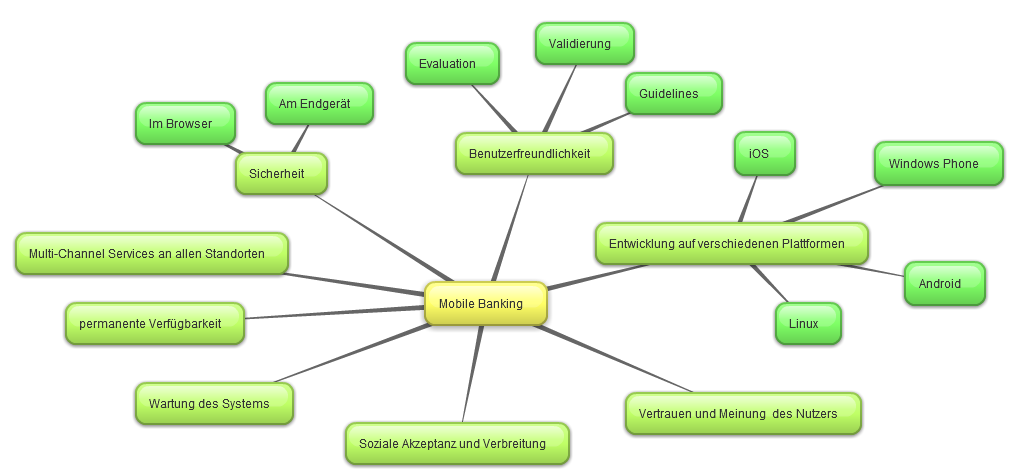
\includegraphics[width=16cm, height=10cm]{figures/mm_mobilebanking}
\end{figure}

\begin{figure}[h!]
	\centering
	\caption{Mindmap Cloud Computing}
		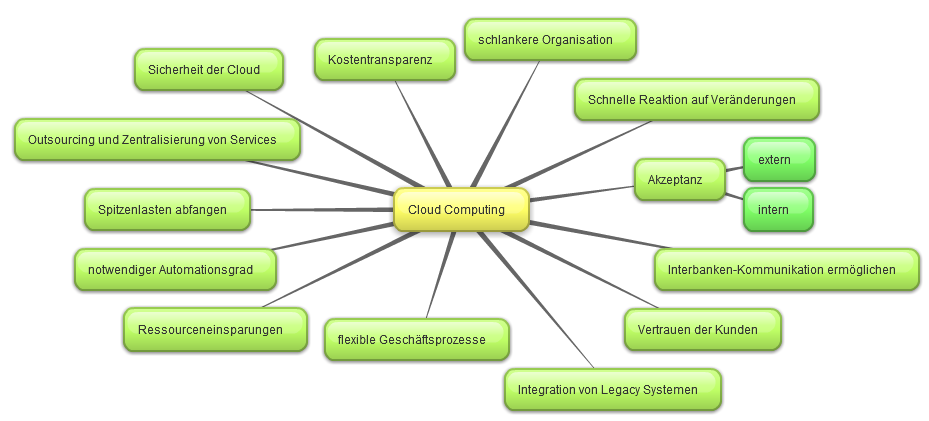
\includegraphics[width=16cm, height=9cm]{figures/mm_cloudcomputing}
\end{figure}

\begin{figure}[h!]
	\centering
	\caption{Mindmap Contactless Payment}
		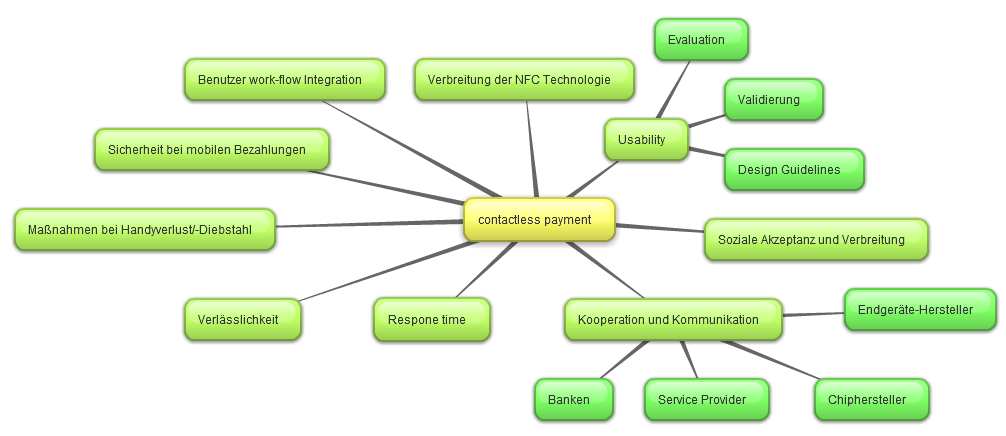
\includegraphics[width=16cm, height=9cm]{figures/mm_contactlesspayment}
\end{figure}

\newpage
\textbf{Vision \& Ziele}\\
Auf Basis der gefundenen Herausforderungen f�r das Unternehmen wurden die folgenden vier Ziele definiert welche mit einer IT-Strategie erreicht werden sollen. 

\begin{enumerate}
	\item Mobiles und intuitives Banking f�r die Kunden, anywhere and anytime.

	\item Wirtschaftliche Flexbilit"at dur smarte und skalierbare IT-Infrastruktur.
	
	\item Innovationsf"uhrerschaft durch die Bezahltechniken von Morgen.
	
	\item Vertrauensbildung bei Kunden und Mitarbeitern durch bei allen Innovationen und Produkten.
\end{enumerate}

\textbf{Generelle Strategien}
\begin{enumerate}

	\item Einf"uhrung eines kundenfreundlichen und mobilen Banking-Portales, welches auf allen Ger�ten funktioniert und den Kunden eine breite Palette an n"utzlichen Features bietet.\\
\textbf{TBW Markus}

	\item Einf"uhrung eines zentralen Cloud-Systems welches die notwendigen internen Services ''on demand'' allen Standorten zu Verf"ugung stellt. \\
\textbf{TBW Christoph }

	\item Bankomatkarte mit NFC Technologie ausr�sten, embedded Bankomatkarte am Handy, Partner und Vertr�ge f�r Chipkarten und Endger�te in Gesch�ften.\\
\textbf{TBW Li}

	\item Sicherheit, Verf"ugbarkeit und Verl"asslichkeit in allen Systemen.\\
\textbf{TBW Anton}

\end{enumerate}









